\RequirePackage[hyphens]{url}
\documentclass[11pt,a4paper,titlepage]{article}
\usepackage[a4paper, top=2.5cm, bottom=2.5cm, left=2.5cm, right=3cm]{geometry}
\usepackage[utf8]{inputenc}
\usepackage[english]{babel}
\usepackage{lipsum}
\usepackage{graphicx}
\graphicspath{ {./pics/} {./eps/}}
\usepackage{epsfig}
\usepackage{epstopdf}
\newcommand\tab[1][1cm]{\hspace*{#1}}
\usepackage{newfloat}
\usepackage{float} %img floats
\usepackage{parskip}
\usepackage{tabularx}
\usepackage{enumitem} %fancy itemize list
\usepackage{multirow}
\usepackage{float}
\usepackage{longtable}

%% FLOAT TYPES
\DeclareFloatingEnvironment[name={Appendix}]{Appendix}

%% COLOR DEFINITIONS
\usepackage[svgnames]{xcolor} % Enabling mixing colors and color's call by 'svgnames'
\definecolor{MyColor1}{rgb}{0.2,0.4,0.6} %mix personal color
\newcommand{\textb}{\color{Black} \usefont{OT1}{lmss}{m}{n}}
\newcommand{\blue}{\color{MyColor1} \usefont{OT1}{lmss}{m}{n}}
\newcommand{\blueb}{\color{MyColor1} \usefont{OT1}{lmss}{b}{n}}

%% SECTIONS
\usepackage{titlesec}
\usepackage{sectsty}
\usepackage{csquotes}

% CAPTIONS AND REFERENCING
\usepackage{caption}
\usepackage{subcaption}
\usepackage{nameref}

%% BIBLIOGRAPHY SETTINGS
\usepackage[style=authoryear,backend=biber,uniquename=init,urldate=long,giveninits=true]{biblatex}
\setlength\bibitemsep{\baselineskip}
\addbibresource{bibliography.bib}
\DeclareNameAlias{sortname}{family-given}
\DeclareNameAlias{default}{family-given}

%% DESIGN CIRCUITS
\usepackage[siunitx, american, smartlabels, cute inductors, europeanvoltages]{circuitikz}

%% APPENDIX SETTINGS
\usepackage[toc,page,title]{appendix}
\renewcommand\appendixtocname{Appendices}
\renewcommand\appendixpagename{Appendices}

%% INCLUDE PDF
\usepackage{pdfpages}

%% CODE SNIPPET LISTING SETTINGS
\usepackage{listings}
\renewcommand\lstlistlistingname{List of Listings}
\lstset{numbers=left,xleftmargin=2em,captionpos=b}
%%Listing style for java.
\definecolor{dkgreen}{rgb}{0,0.6,0}
\definecolor{gray}{rgb}{0.5,0.5,0.5}
\definecolor{mauve}{rgb}{0.58,0,0.82}
\lstset{frame=tb,
	language=Java,
	aboveskip=3mm,
	belowskip=3mm,
	showstringspaces=false,
	columns=flexible,
	basicstyle={\small\ttfamily},
	numbers=left,
	numberstyle=\tiny\color{gray},
	keywordstyle=\color{blue},
	commentstyle=\color{dkgreen},
	stringstyle=\color{mauve},
	breaklines=true,
	breakatwhitespace=true,
	tabsize=3
}

\lstdefinelanguage{JavaScript}{
  keywords={break, case, catch, continue, debugger, default, delete, do, else, false, finally, for, function, if, in, instanceof, new, null, return, switch, this, throw, true, try, typeof, var, void, while, with},
  morecomment=[l]{//},
  morecomment=[s]{/*}{*/},
  morestring=[b]',
  morestring=[b]",
  ndkeywords={class, export, boolean, throw, implements, import, this},
  keywordstyle=\color{blue}\bfseries,
  ndkeywordstyle=\color{darkgray}\bfseries,
  identifierstyle=\color{black},
  commentstyle=\color{purple}\ttfamily,
  stringstyle=\color{red}\ttfamily,
  sensitive=true
}

\colorlet{punct}{red!60!black}
\definecolor{delim}{RGB}{20,105,176}
\colorlet{numb}{magenta!60!black}

\lstdefinelanguage{json}{
    basicstyle=\normalfont\ttfamily,
    numbers=left,
    numberstyle=\scriptsize,
    stepnumber=1,
    numbersep=8pt,
    showstringspaces=false,
    breaklines=true,
    frame=lines,
    literate=
     *{0}{{{\color{numb}0}}}{1}
      {1}{{{\color{numb}1}}}{1}
      {2}{{{\color{numb}2}}}{1}
      {3}{{{\color{numb}3}}}{1}
      {4}{{{\color{numb}4}}}{1}
      {5}{{{\color{numb}5}}}{1}
      {6}{{{\color{numb}6}}}{1}
      {7}{{{\color{numb}7}}}{1}
      {8}{{{\color{numb}8}}}{1}
      {9}{{{\color{numb}9}}}{1}
      {:}{{{\color{punct}{:}}}}{1}
      {,}{{{\color{punct}{,}}}}{1}
      {\{}{{{\color{delim}{\{}}}}{1}
      {\}}{{{\color{delim}{\}}}}}{1}
      {[}{{{\color{delim}{[}}}}{1}
      {]}{{{\color{delim}{]}}}}{1},
}

%% PAGE HEADER STYLING
\usepackage{etoolbox,fancyhdr,xcolor}

%% ACRONYMS
\usepackage{acronym}


%%%%%%%%%%%%%%%%%%%%%%%%%%%%%%%%%%%%%%%%%%%%%%%%%%
%% START OF DOCUMENT
%%%%%%%%%%%%%%%%%%%%%%%%%%%%%%%%%%%%%%%%%%%%%%%%%%


%% TITLE PAGE SETTINGS
\title{\textbf{End-To-End Testing for React Native Applications} \\
Research Report}
\author{Sebastian Wilczek}
\date{\vspace*{\fill} Fontys University of Applied Sciences\\ \bigskip Venlo, \today}

\begin{document}

%% CONFIGURATION OF PAGE HEADER
\pagestyle{fancy}
\newcommand{\headrulecolor}[1]{\patchcmd{\headrule}{\hrule}{\color{#1}\hrule}{}{}}
\newcommand{\footrulecolor}[1]{\patchcmd{\footrule}{\hrule}{\color{#1}\hrule}{}{}}
\pagestyle{fancy}
\fancyhf{}% Clear header/footer
\fancyhead[C]{}
\fancyhead[R]{\thepage}
\setlength{\headsep}{33pt}
\setlength{\headheight}{13.6pt}
\renewcommand{\headrulewidth}{0.4pt}


%%%%%%%%%%%%%%%%%%%%%%%%%%%%%%%%%%%%%%%%%%%%%%%%%%
%% START OF CONTENT
%%%%%%%%%%%%%%%%%%%%%%%%%%%%%%%%%%%%%%%%%%%%%%%%%%


%% TITLE PAGE
\maketitle
\newpage

%% SET PAGE NUMBERING TO ROMAN
\pagenumbering{roman}
\setcounter{page}{2}

%% INFORMATION PAGE
%% \include{content/informationPage}

%% SUMMARY
\section*{Summary}
\addcontentsline{toc}{section}{Summary}

In recent mobile application development, the \textit{React Native} framework has gathered a large following because of it's cross-platform deployment approach. Developing and moving applications to production is made rather easy with the framework, both for the aforementioned cross-platform compatibility as well as the large availability of open source components that are free to use and offered on the internet.
\newline
However, a part often overlooked in \textit{React Native} development is testing. Many developers use manual testing on their applications by deploying them to testing devices or emulators while simply executing the actions a user would. This makes the development inefficient and the product unreliable due to the possibility of non-tested errors.
\newline
This research aims to answer the question how applications developed in \textit{React Native} can be tested properly, more specifically how end-to-end testing can be applied successfully in such a project. To do so, a collection of potential end-to-end testing frameworks is considered under defined circumstances, such as cross-platform compatibility, ease of use and necessary change to production code.
\newline
The testing framework are tested in the context of a project working on the application \textit{Connected.Football}. Conclusions are drawn both as to whether the testing frameworks are applicable to the project in question as well as how they can be used in a general \textit{React Native} project that is tested from the very beginning.

%% STATEMENT OF AUTHORSHIP
%% \addcontentsline{toc}{section}{Statement of Authenticity}

\includepdf[pages=-]{stmtOfAuthorship} 

%% TABLE OF CONTENT
\tableofcontents
\newpage

%% LIST OF FIGURES
\addcontentsline{toc}{section}{List of Figures}
\listoffigures
\newpage

%% LIST OF TABLES
%% \addcontentsline{toc}{section}{List of Tables}
%% \listoftables
%% \newpage

%% LIST OF LISTINGS
\addcontentsline{toc}{section}{List of Listings}
\lstlistoflistings 
\newpage

%% LIST OF ABBREVIATIONS
\addcontentsline{toc}{section}{List of Abbreviations}
\section*{List of Abbreviations}
\begin{acronym}[MPC] % Give the longest label here so that the list is nicely aligned
\acro{ADB}{Android Debug Bridge}
\acro{AVD}{Android Virtual Device}
\acro{API}{Application Programming Interface}
\acro{HTTP}{Hypertext Transfer Protocol}
\acro{LLC}{Limited Liability Company}
\acro{OS}{Operating System}
\acro{UI}{User Interface}
\end{acronym}
\newpage

%% SET PAGE NUMBERING TO ARABIC
\pagenumbering{arabic}
\setcounter{page}{1}

%% INTRODUCTION
\section{Introduction}
\label{sec:introduction}
\lhead{\thesection \space Introduction}

This document is a research report on the topic of end-to-end testing of \textit{React Native} applications. \textit{React Native} is a framework developed by Facebook that enables developers to write one singular base of \textit{JavaScript} development code for a mobile based application and to then deploy them to various mobile platforms, predominately \textit{Android} and \textit{iOS}. The framework itself is based on \textit{ReactJS} and is handled similarly (\cite{react-native}).
\newline
The research was conducted as part of a development project involving the mobile application \textit{Connected.Football}, which is being developed using \textit{React Native}. During development, the question came up as to how such an application can be properly tested, especially how it can be assured that a user of the application is able to use it as intended.
\newline
The following chapters will first of all detail how the research was planned to be conducted. To illustrate that, it will be defined why the research was done in the first place, what questions were asked and answered, and what methods were to be made use of during the research.
\newline
What follows are the results of the research. The results contain mostly a collection of different testing frameworks and their advantages when compared to others. Each framework is tested regarding the requirements necessary, as they are defined by the project work and the environment of the \textit{Connected.Football} application. The result chapter also contains sample code written for some of the researched framework. Furthermore, it is explained how the frameworks could be used in the application development in question as well as in general \textit{React Native} development.
\newline
The report ends with a conclusion, summarising the results of the research and giving advice as to how the testing frameworks are to be used in the project. It also contains general advice as to how to approach \textit{React Native} end-to-end testing.

%% RESEARCH DEFINITION
\section{Research Definition}
\label{sec:research_definition}
\lhead{\thesection \space Research Definition}

This chapter contains details as to how the research was conducted. This includes an explanation as to why the research was necessary in the first place as well as a set of questions that the research aims to answer. Furthermore, it is detailed what kind of research methods were made use of during the research.

\subsection{Research Motivation}
\label{ssec:research_motivation}

The research is part of a project on the \textit{Connected.Football} mobile application. The application itself is developed using \textit{React Native}, a frontend framework developed by Facebook (\cite{react-native}).
\newline
During development, the development team realised that they do a lot of manual testing, as in continuously going through the same repetitive steps to test certain use cases, for example entering an email and a password every time they want to test something that requires a user to be logged in. Eventually, the question came up as to how this form of testing can be done more efficiently, since the developers lose a huge amount of time testing repetitive interactions. Furthermore, due to the repetitive nature of such tests, the developers may overlook some flaws in the developed product, which could also be avoided through proper tests.

\subsection{Research Questions}
\label{ssec:research_questions}

As a guideline of what should be researched, the following research questions were defined:

\begin{enumerate}
\item How can React Native applications be end-to-end tested?
\item What framework is the best to use for the React Native application in question?
\begin{enumerate}
\item Does it fit the development environment?
\item Is it easy to use, in terms of setup, test development and execution?
\item Is it compatible with the already existing product?
\end{enumerate}
\item Is end-to-end testing a feasible thing to do in the project in question?
\end{enumerate}

\subsection{Research Methods}
\label{ssec:research_methods}

To answer the aforementioned questions and to conduct the research, a set of methods is to be made use during the research. First of all, the research conduction will include mostly literature research. It will be researched what frameworks are available and what the advantages and disadvantages to using them are. Literature to be used comes from the official documentations of the various frameworks as well as by publications of developers making use of specific frameworks.
\newline
Furthermore, interviews with the \textit{React Native} developers of the project in question are to be conducted. The interview topics will be how testing is currently done in development, how it could be made more efficient, what their development environment is like when it comes to for instance operating systems and whether or not existing code should be changed or more work put into future development for the sake of testing.

\subsection{Interview Questions}
\label{ssec:interview_questions}

As mentioned in \textit{Chapter \ref{ssec:research_methods}}, an interview with \textit{React Native} developers is part of the research methods applied. The following questions are to be asked to the developers and answers to said questions will be referenced in the coming chapter.

\begin{enumerate}
\item How do you currently test artefacts developed in \textit{React Native}?
\item Does the testing include any repetitive or unnecessary elements?
\item Could the testing process be made more efficient? If yes, how?
\item What is included in your development environment? (OS, Mobile OS, emulation, physical devices)
\item Is it worth it to change existing code or to put extra work into future work on source code, if tests can be made more accessible and easier to use this way?
\end{enumerate}

A transcript of all interviews can be found in the Appendix (see \textit{Appendices \ref{appendix:interview_lucas_gehlen}, \ref{appendix:interview_marco_kull}, \ref{appendix:interview_patrick_richter}}).

%% RESEARCH RESULTS
\section{Research Results}
\label{sec:research_results}
\lhead{\thesection \space Research Results}

The following chapter describes the results that the research brought forth. Structurally, the chapter is made up of sub-chapters detailing a list of various frameworks.
\newline
For each framework, it is described how the framework can be used to test a \textit{React Native} application. Furthermore, depending on the advantages and disadvantages the frameworks brings, it is defined whether or not the framework in question is fit to be used during the \textit{Connected.Football} project.
\newline
As far as the project itself is concerned, the developers work on a variety of operating systems, including \textit{Windows 10}, \textit{Gentoo Linux} and \textit{macOS 12 Mojave}, according to the interviews conducted with the developers. All developers furthermore deploy and test the application using an \textit{Android} based device or emulator. The developers would like the tests to make their work more efficient, by removing unnecessary repetition and navigation. Having additional unit tests to the end-to-end tests would also be an advantage (see \textit{Appendices \ref{appendix:interview_lucas_gehlen}, \ref{appendix:interview_marco_kull}, \ref{appendix:interview_patrick_richter}}).

\subsection{Jest}
\label{ssec:jest}

\textit{Jest} is the testing framework that is automatically installed whenever a new \textit{React Native} app is created. It is also developed by Facebook. Since version 14, \textit{Jest} is able to create so-called snapshots. Snapshots are records of how a certain part of an application rendered the last time the tests ran successfully. This means that to test using \textit{Jest}, it is defined what component is to be tested with certain properties. If this test has never run, the resulting component rendering tree is stored as a snapshot. If a snapshot already exists, the new rendering tree is compared against it, marking the differences to the snapshot. If the changes are intentional, the developer can store the result as a new snapshot. Ideally, these snapshots should always be committed and stored together with the sources. (\cite{testing-react-native})
\newline
The benefit to using \textit{Jest} is that it is completely platform-independent. What is tested is the generated \textit{React Native} rendering tree, rather that how the platform it is deployed on interprets it. Furthermore, the tests are not dependent on any emulation of an actual device: \textit{"Because tests are run in a command line runner instead of a real browser or on a real phone, the test runner doesn’t have to wait for builds, spawn browsers, load a page and drive the UI to get a component into the expected state which tends to be flaky and the test results become noisy."} (\cite{testing-react-native-with-jest})
\newline
Furthermore, due to not being dependent on a platform, it is also rather simple to provide information that is not accessible through other means, for instance through mocking. State, properties and other values can be given to the tests instead of having to simulate them. This has the advantage than rather to having to replicating state logic in the tests, this logic can also be tested. (\cite{learning-test-react-native})
\newline
However, despite the aforementioned advantages, \textit{Jest} is most useful when testing single components or at most somewhat high-level components. This makes it most useful for unit and component testing. End-to-end testing is rather hard to do with a framework that can only compare old versions of components to new ones. Ideally, \textit{Jest} would have to compare snapshots after executing a chain of commands that are processed by the application that is to be tested. This is also the reason why \textit{Jest} is used in a similar way in some of the testing frameworks mentioned below.

\subsection{Appium}
\label{ssec:appium}

\textit{Appium} is an end-to-end testing framework which uses \textit{Selenium} as a base. Since it was \textit{".. released even before React.js, [making it] the number one in the industry"} (\cite{detox-vs-appium}), it gathered a large following both of \textit{React Native} developers as well as developers using it in different environments. Similar to \textit{Detox}, it makes use of a selection API which sends inputs to specified parts of the application, which is running in an emulator. \textit{Appium} is also able to run tests on actual devices. If an \textit{Android} device is connected to the development machine, \textit{"providing there is only a single device connected, the test will pick up that device for execution."} (\cite[p. 169]{test-automation-appium})
\newline
To run \textit{Appium}, a service is started which connects to the emulator. This service is responsible for propagating the inputs to the actual app. The service itself is actually an HTTP server, as seen in \textit{Figure \ref{fig:appium_server}}, developed in \textit{Node.js} which creates \textit{WebDriver} sessions (\cite{appium-and-selenium}). These sessions can be used by client applications which use certain drivers, depending on the programming language the tests are written in. To test the project in question, the tests are written in \textit{JavaScript}, just like the actual application is. The driver that was made use of is \textit{Webdriver.IO} which comes with its own selection API (\cite{webdriverio}).

\begin{figure}[H]
    \begin{center}
        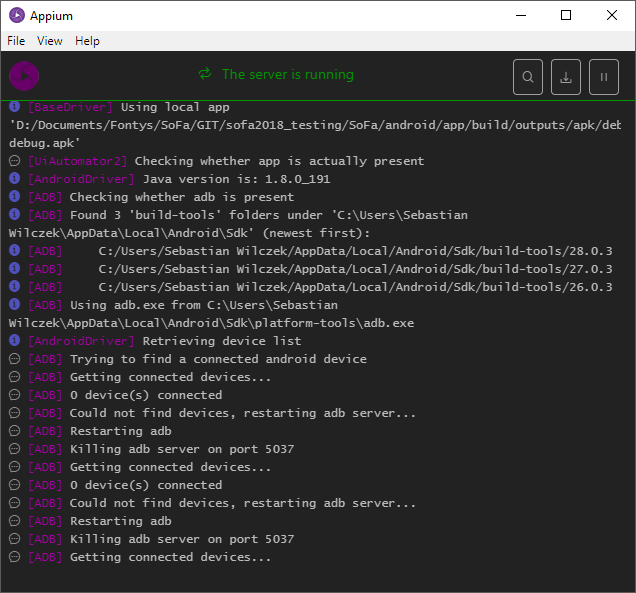
\includegraphics[width=0.9\textwidth]{images/appium_server.png}
        \caption{\textit{Appium} Server}
        \label{fig:appium_server}
    \end{center}
\end{figure}

\newpage

Defining tests in \textit{Appium} is simple. As seen in \textit{Listing \ref{lst:appiumTest}}, test cases can be described which in turn contain instructions on how to interact with the application, or rather how the \textit{Appium} service should interact, including setup and tear down functions to start and end sessions with the service. The actual definition of interaction can make use of the driver's selection API. In the case of testing with \textit{Appium}, this selection is limited to so-called \textit{Accessibility Labels}. These labels are defined in the \textit{React Native} source code and can be read in an \textit{Appium} test using the '\textit{\~}' character

\begin{lstlisting}[language=javascript,caption=\textit{Appium WebdriverIO} Test Example,label=lst:appiumTest]
describe("Basic Android interactions", function() {
  let client;

  beforeEach(function() {
    client = webdriverio.remote(opts);
    return client.init().pause(15000);
  });

  afterEach(function() {
    return client.end();
  });

  it("should click a tab that opens more functionality", async function() {
    return client
      .waitForExist('~More', 5000)
      .element('~More')
      .click()
      .waitForExist("~Privacy", 5000)
      .getText("~Privacy", function(result) {
        assert.equal(result.value, "Privacy");
      });
  });
});
\end{lstlisting}

Using the labels has two major downsides. First of all, the development team would be forced to create such an identification for each element that would be involved in the testing process. As stated in the interviews, it would be preferable to test using as little change to actual developed work as necessary.
\newline
Furthermore, the \textit{Accessibility Label} is also exposed to the user. In the accessibility options of \textit{Android}, it is possible to enable a setting that enables screen reading applications to read out the functions of an application to vision-impaired users, as described by the aforementioned labels. (\cite{accessible-apps})
\newline
Unfortunately, the labels are also the reason why the testing framework can not be applied to the project in question. While it was possible to define and execute tests using \textit{Appium}, including interacting with the application, the application also makes use of various open source \textit{React Native} components which do not support the usage of \textit{Accessibility Labels}. In particular, the module \textit{react-native-navigation} caused problems this way, making it impossible for tests to ever leave the starting view of the application.

\subsection{Espresso}
\label{ssec:espresso}

\textit{Espresso} is a library developed and maintained by Google designed for \textit{Android} test automation (\cite{appium-pro}). Since it is developed only for \textit{Android}, it can not be used to test applications running on an \textit{iOS} device or emulator.
\newline
The testing framework was developed having \textit{Android} native applications in mind, with the possibility of testing \textit{React Native} applications added later on. Given this change, \textit{Espresso} was also made available to be used as a driver for \textit{Appium}, similar to \textit{Webdriver.IO} and \textit{UIAutomator2}, which is also developed by Google.
\newline
An advantage of using \textit{Espresso} is the way it manages timing while interacting with the application. \textit{"Espresso requires no waiting method calls to ensure synchronization of the UI, [making it] clearly [one of] the fastest of the tools"} (\cite{comparison-gui}).
\newline
However, in the same way as \textit{Appium}, the framework is only able to access components through given identification, which is again defined through labels. This again makes it impossible to use \textit{Espresso} in the given project. For detailed information about the problem posed by the \textit{Accessibility Labels}, see \textit{Chapter \ref{ssec:appium} \nameref{ssec:appium}}.

\subsection{Detox}
\label{ssec:detox}

\textit{Detox} is another testing framework that simulates user interaction. Originally it was developed to run only on \textit{macOS} and \textit{iOS} platforms. Recently, the developers decided to make the framework available to \textit{Android} developers as well, releasing in-development artefacts as they are continuing to make it fully functional. (\cite{android-status})
\newline
Similar to \textit{Espresso}, \textit{Detox} tries to improve test stability using a gray box approach, by only running interactions once other interactions have been processed and the application is running in an idle state. \textit{Figure \ref{fig:detox_check}} shows the check performed by \textit{Detox} every few milliseconds. The framework will wait until it is asserted that the application's resources are running in an idle state or until a callback makes \textit{Detox} run regardless.

\begin{figure}[H]
    \begin{center}
        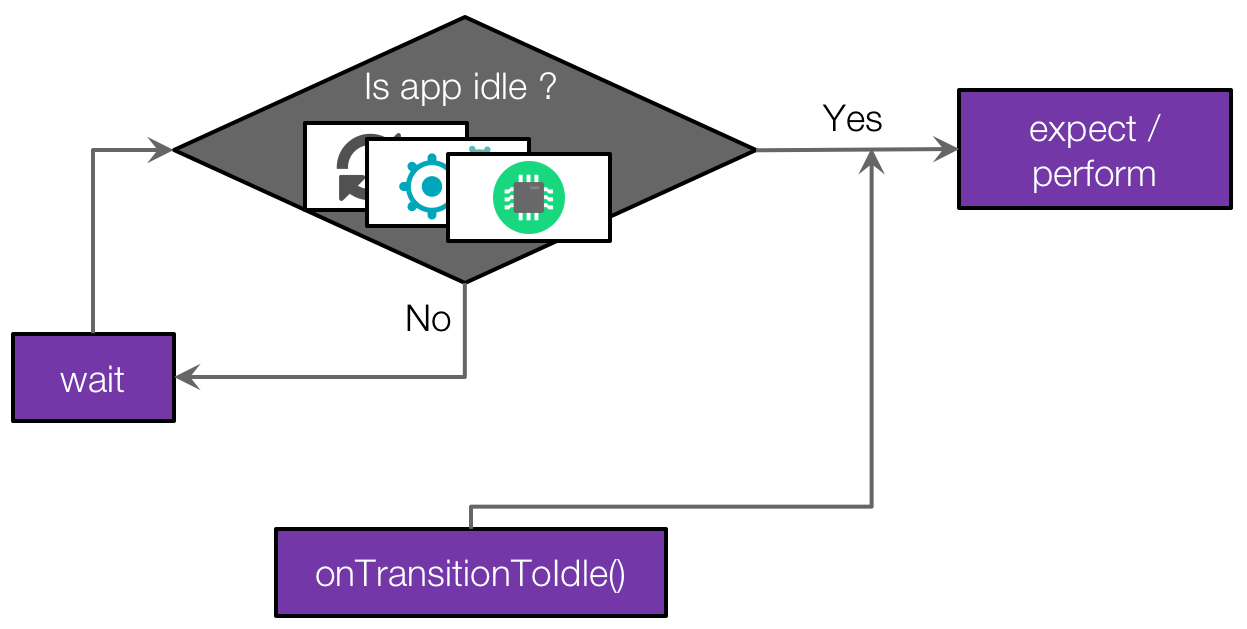
\includegraphics[width=0.8\textwidth]{images/detox_check.png}
        \caption{\textit{Detox} Idle State Check (\cite{detox-gray-box})}
        \label{fig:detox_check}
    \end{center}
\end{figure}

\newpage

\textit{Detox} is very simple to setup and use in a project. Once it has been installed as part of the modules of a \textit{React Native} project, multiple configurations can be created to test in different environments, such as different devices running \textit{Android} and \textit{iOS}. \textit{Listing \ref{lst:detoxConfig}} shows two such configurations.

\begin{lstlisting}[language=json,caption=\textit{Detox} Configuration Example,label=lst:detoxConfig]
"detox": {
  "configurations": {
    "ios.sim.debug": {
      "binaryPath": "ios/build/Build/Products/Debug-iphonesimulator/example.app",
      "build": "xcodebuild -project ios/example.xcodeproj -scheme example -configuration Debug -sdk iphonesimulator -derivedDataPath ios/build",
      "type": "ios.simulator",
      "name": "iPhone 7"
    },
    "android.emu.debug": {
      "binaryPath": "android/app/build/outputs/apk/debug/app-debug.apk",
      "build": "cd android && gradlew assembleDebug assembleAndroidTest -DtestBuildType=debug && cd ..",
      "type": "android.attached",
      "name": "emulator_5554"
    }
  },
  "test-runner": "jest"
}
\end{lstlisting}

These configurations include definitions on how to run the test builds as well as on what platform to run them. For instance, the second configuration run the test using ADB on an \textit{Android} device with the name \textit{emulator\_5554}, which in this case is the running AVD emulator.
\newline
Just like most other frameworks, \textit{Detox} has an API to select components. However, there is at the time of writing no documentation that details how this API can be used with a \textit{React Native} application that is built for and deployed to an \textit{Android} device. It could however be assumed that it might have to rely on \textit{Accessibility labels}, just like \textit{Appium}.
\newline
Furthermore, when trying to run an example test, just to see if it fails, \textit{Detox} failed to run with multiple different errors depending on the chosen configuration. No documentation or reproduction of these errors could be found either. It is not known if the low support and early development stage of the \textit{Android} functionality or the compatibility to the given project is to blame, however, the high amount of errors with no apparent solution makes \textit{Detox} unsuitable for the project, despite being a promising product.

\subsection{Cavy}
\label{ssec:cavy}

\textit{Cavy} is the newest available framework to test \textit{React Native} applications at the time of writing. It tests applications by running an application in a simulated environment, in the same way \textit{Appium} and \textit{Detox} does, finding components using a selection API and interacting with them in a specified way.
\newline
The difference between \textit{Cavy} and other similar tools is the way it finds and accesses components. The most notable \textit{".. difference is that Appium uses native hooks to access components (accessibility IDs), wheras [sic] Cavy uses React Native refs. This means that Cavy sits directly within your React Native environment [...] without much overhead."} (\cite{cavy})
\newline
While it is a good idea to use only functionality that is already available in the \textit{React Native} framework, this also means that every component that has to be tested has to be marked as such. To do so, \textit{"Cavy (ab)uses React ref generating functions to give you the ability to refer to, and simulate actions upon, deeply nested components within your application."} (\cite{cavy})
\newline
In other terms, that means that every component written in \textit{React Native} needs to include a specific syntax when used. This syntax appears to be rather complicated, as shown in \textit{Listing \ref{lst:cavyHook}}, and can become hard to read when used in many components.

\begin{lstlisting}[language=javascript,caption=\textit{Cavy} Hook Example,label=lst:cavyHook]
<TextInput
  ref={this.props.generateTestHook('Scene.TextInput')}
  onChangeText={...}
/>
\end{lstlisting}

There is a small workaround available to make the source code more readable. This workaround makes use of \textit{Higher-Order Components}, which \textit{"is an advanced technique in React for reusing component logic"} (\cite{hoc}). Making use of this technique, the rather complex looking syntax can be replaced by the word \textit{testable} and the name of the components to be referenced with. Essentially this is the same as the previous syntax, just far more readable. (\cite{e2e_cavy})
\newline
In any case, the entire app must also be wrapped in a test related component, which receives the testing hooks. This another change to production code that is undesirable.
\newline
While the creation of test hooks looks rather complicated, the definition of tests is rather simple. The selection API provides, even if it is a bit simplistic, enough ways to select and interact with \textit{React Native} components. An example test script can be found in \textit{Listing \ref{lst:cavyTest}}.

\begin{lstlisting}[language=javascript,caption=\textit{Cavy} Test Example,label=lst:cavyTest]
export default function(spec) {
  spec.describe('My feature', function() {
    spec.it('works', async function() {
      await spec.fillIn('Scene.TextInput', 'some string')
      await spec.press('Scene.button');
      await spec.exists('NextScene');
    });
  });
}
\end{lstlisting}

While \textit{Cavy} looks great in theory, aside from the massive change to the existing source code, it is not possible to make use of it in the project in question. The project makes heavy use of functional components, and since \textit{"functional components cannot be assigned a ref since they don't have instances"} (\cite{cavy}), \textit{Cavy} will not be able to access these components. Using \textit{Recompose}, it might be possible to convert functional components to \textit{React Native} classes, however that is more change to existing code and goes against the principle and goal of functional components.

%% CONCLUSION
\section{Conclusion}
\label{sec:Conclusion}
\lhead{Conclusion}

As part of this research, many testing frameworks were considered whether they are easy and efficient to test with and if their usage is applicable in the project in question. According to the interviews conducted with \textit{React Native} developers working on the project, this means that the framework should ideally be cross-platform compatible both for the mobile OS, as in \textit{Android} and \textit{iOS}, although \textit{Android} is the preferred platform, as well as the development platform, meaning \textit{Windows}, \textit{Linux} and \textit{mac OS}. Furthermore, the framework should require as little change to the source code as possible, both to existing code as well as how code should be written in the future of the project.
\newline
All examined platforms have their advantages and disadvantages. However, the research results in the conclusion that, at least for the project in question, none of the testing frameworks can be applied and used in an efficient way.
\newline
\textit{Jest} offers great functionality when it comes to testing singular components. The snapshot feature makes it test at a very high speed without the need for any emulation, and it's platform independence makes it usable almost everywhere in the context of \textit{React Native}. However, the framework was designed with a more component-based testing approach in mind, and it is best used that way. The simulation of user input and information processing can not be created in a test environment using only \textit{Jest}.
\newline
\textit{Appium} has the advantage of having a great interaction API and tests that are easily readable. It is also able to run cross-platform. However, the dependency on \textit{Accessibility Labels} makes it incompatible with some \textit{React Native} components, as it is the case with the already developed product. Furthermore, using the labels is more change to the source code and also indirectly perceivable by the user of the application.
\newline
\textit{Espresso} does have a good approach with it's synchronisation. However, this feature is also available in other frameworks, for instance \textit{Detox}, and it might not be the most up-to-date framework available. It's limitation to the Android platform also makes it less than ideal.
\newline
\textit{Detox} combines the easy usability of \textit{Appium} and the great synchronisation features of \textit{Espresso}. It is also simple to set up, offering the possibility of defining many different testing configurations. However, the API is more limited than the one of \textit{Appium} and, same as \textit{Appium}, components are not recognised during the testing procedure. For now, the functionality is also limited when it comes to the \textit{Android} platform.
\newline
Lastly, \textit{Cavy} has a great approach when referencing components when one thinks about performance, since the references used by \textit{Cavy} are only making use of the \textit{React Native} framework, instead of native platform identification. However, just like \textit{Appium} and \textit{Detox}, this requires every component to be marked as a testable component during development, making the selection API very limited, with the added disadvantage of needing to wrap the entire application in a test hooking function. Furthermore, \textit{Cavy} does not support functional components, another paradigm that is made heavily use of in the project in question.
\newline
For the reason reiterated above, no testing framework is completely applicable to the project. However, if one were to create a new \textit{React Native} application, the following suggestions could be made:
\newline
Every major component should be unit or component tested making use of \textit{Jest}'s snapshot feature. For end-to-end testing, developers should decide between \textit{Appium} and \textit{Detox}, depending on the needed complexity of the written tests, with \textit{Appium} for more complex tests. If the required complexity level of tests is not as high, \textit{Detox} can be used for the sake of an easy setup and configuration. In any case, it should be paid attention to the fact that the components that are made use of need to be able to be referenced by the chosen test framework, for example through \textit{Accessibility Labels}. If it can be made sure that no functional components will ever be used as part of the application, \textit{Cavy} may also be used as an alternative.
\newline
Overall, each testing framework does what it is intended to do, which is testing a \textit{React Native} application. This research has returns some of the caveats and disadvantages of the tested frameworks. However, it also shows some of the positive aspects of each as well as potential reasons why and environments to use them in. One thing that can be taken away from this research is that testing is a part of software development that should be considered from the very beginning of a project, even when working with a very frontend focused framework such as \textit{React Native}. Introducing tests late in a project results mostly in errors and compatibility issues, like it did in this project. If tests are written and executed properly from the start, both the product and the tests written for it can develop into software that works as intended.

%% BIBLIOGRAPHY
\newpage
\addcontentsline{toc}{section}{List of References}
\lhead{List of References}
\printbibliography{}

%% APPENDIX
\newpage
\lhead{Appendices}
\patchcmd{\appendices}{\quad}{: }{}{}
\begin{appendices}

%\addcontentsline{toc}{section}{Appendix A: Interview Lucas Gehlen}
\section{Interview Lucas Gehlen}
\label{appendix:interview_lucas_gehlen}

The following is a transcript of the interview conducted with the \textit{React Native} developer Lucas Gehlen. Formalities at the beginning and the end of the interview that are not related to any relevant information have been omitted from the transcript.
\newline
\newline
\textbf{Interviewer:} How do you currently test artefacts developed in \textit{React Native}?
\newline
\newline
\textbf{L. Gehlen:} I don't, really. All I do is manually enter actions and values into the application to test certain use cases.
\newline
\newline
\textbf{Interviewer:} Does the testing include any repetitive or unnecessary elements?
\newline
\newline
\textbf{L. Gehlen:} Yes. I often run through the same actions to test the same cases over and over again, wasting time.
\newline
\newline
\textbf{Interviewer:} Could the testing process be made more efficient? If yes, how?
\newline
\newline
\textbf{L. Gehlen:} Probably. I don't really know how though.
\newline
\newline
\textbf{Interviewer:} What is included in your development environment? (OS, Mobile OS, emulation, physical devices)
\newline
\newline
\textbf{L. Gehlen:} I use \textit{macOS 10 Sierra} on my development machine, as well as \textit{Android 8 on an Android Emulator}. I do not use any physical devices.
\newline
\newline
\textbf{Interviewer:} Is it worth it to change existing code or to put extra work into future work on source code, if tests can be made more accessible and easier to use this way?
\newline
\newline
\textbf{L. Gehlen:} No, it is not worth it and way too much effort.

\newpage

\section{Interview Marco Kull}
\label{appendix:interview_marco_kull}

The following is a transcript of the interview conducted with the \textit{React Native} developer Marco Kull. Formalities at the beginning and the end of the interview that are not related to any relevant information have been omitted from the transcript.
\newline
\newline
\textbf{Interviewer:} How do you currently test artefacts developed in \textit{React Native}?
\newline
\newline
\textbf{M. Kull:} I only test by hand, using the application like a normal user would, to see if it works as intended. Very tedious.
\newline
\newline
\textbf{Interviewer:} Does the testing include any repetitive or unnecessary elements?
\newline
\newline
\textbf{M. Kull:} Yes, I have to wait very long times for the application to be deployed to a device before it is ready. It takes forever to navigate to the things I want to test.
\newline
\newline
\textbf{Interviewer:} Could the testing process be made more efficient? If yes, how?
\newline
\newline
\textbf{M. Kull:} Yes. A more clear separation of functionality and user interface is needed, this way it would also be possible to do unit testing, which would be nice. It would be great if the navigation could be quicker by using tests.  
\newline
\newline
\textbf{Interviewer:} What is included in your development environment? (OS, Mobile OS, emulation, physical devices)
\newline
\newline
\textbf{M. Kull:} I run \textit{Gentoo Linux} and I have a physical \textit{Nexus 6 P} device running \textit{Android 8}. 
\newline
\newline
\textbf{Interviewer:} Is it worth it to change existing code or to put extra work into future work on source code, if tests can be made more accessible and easier to use this way?
\newline
\newline
\textbf{M. Kull:} Yes. In a professional setting this should be done in a certain extent, as long as the process of doing so does not put unnecessary strain on the development team.

\newpage

\section{Interview Patrick Richter}
\label{appendix:interview_patrick_richter}

The following is a transcript of the interview conducted with the \textit{React Native} developer Patrick Richter. Formalities at the beginning and the end of the interview that are not related to any relevant information have been omitted from the transcript.
\newline
\newline
\textbf{Interviewer:} How do you currently test artefacts developed in \textit{React Native}?
\newline
\newline
\textbf{P. Richter:} I don't test at all.
\newline
\newline
\textbf{Interviewer:} Does the testing include any repetitive or unnecessary elements?
\newline
\newline
\textbf{P. Richter:} Nope, since I do not test the application.
\newline
\newline
\textbf{Interviewer:} Could the testing process be made more efficient? If yes, how?
\newline
\newline
\textbf{P. Richter:} Yes, of course, there needs to be a lot more testing overall.
\newline
\newline
\textbf{Interviewer:} What is included in your development environment? (OS, Mobile OS, emulation, physical devices)
\newline
\newline
\textbf{P. Richter:} I have \textit{macOS Mojave} and an \textit{Android 8} device, which is a \textit{Nexus 6 P}.
\newline
\newline
\textbf{Interviewer:} Is it worth it to change existing code or to put extra work into future work on source code, if tests can be made more accessible and easier to use this way?
\newline
\newline
\textbf{P. Richter:} Of course, that would be reasonable. Seems alright to me.

\end{appendices}

\end{document}